\begin{chapter}{Control}

    % robust linear control: https://inst.eecs.berkeley.edu/~ee127/sp21/livebook/l_sdp_apps_stability.html
    % AA203 Examples: https://github.com/StanfordASL/AA203-Examples
    % multi target tracking
        % MATLAB: https://www.mathworks.com/videos/sensor-fusion-part-5-how-to-track-multiple-objects-at-once-1569411395828.html 
        % potentially good: https://stonesoup.readthedocs.io/en/v0.1b9/auto_tutorials/06_DataAssociation-MultiTargetTutorial.html
    % Learning convex control policies https://stanford.edu/~boyd/papers/pdf/l4dc_cocp_talk.pdf
    % "" but longer: https://stanford.edu/~boyd/papers/pdf/learning_cocps.pdf
    % real time multiple object tracking for autonomous navigation: https://cs231n.stanford.edu/reports/2017/pdfs/630.pdf
    % Learning to track: https://cvgl.stanford.edu/papers/xiang_iccv15.pdf
    
    \section{Overview}

    % Need to add AA203 overview to this

    % PROBLEMS TO FINISH PRE 6/07/24    
        % Just put in the boeing control problem from VMLS
        % Robot manipulator exercise 18.7 VMLS
        % Boyd 16.2 Optimal Spacecraft landing 
        % path planning with contingencies

    \begin{figure}[h!]
        \centering
        \begin{forest}
            for tree={
                grow=east,
                parent anchor=east,
                child anchor=west,
                edge path={
                    \noexpand\path [draw, \forestoption{edge}]
                    (!u.parent anchor) -- +(5pt,0) |- (.child anchor)\forestoption{edge label};
                },
                l sep+=10pt,
                s sep+=10pt,
                anchor=west,
                align=center
            }
            [Control
                [Passive\\(Optimal Design)]
                [Active
                    [Open Loop]
                    [Closed Loop]
                ]
            ]
        \end{forest}
        \caption{Control Strategies}
        \label{fig:control_tree}
    \end{figure}

    \begin{figure}[h!]
        \centering
        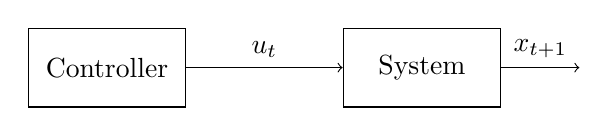
\begin{tikzpicture}[auto, node distance=2cm]
            % Nodes
            \node [draw, rectangle, minimum width=2cm, minimum height=1cm] (control) {Controller};
            \node [draw, rectangle, minimum width=2cm, minimum height=1cm, right of=control, node distance=4cm] (system) {System};
            
            % Arrows
            \draw [->] (control) -- node[above] {$u_t$} (system);
            \draw [->] (system) -- node[above] {$x_{t+1}$} ++(2cm, 0);
    
        \end{tikzpicture}
        \caption{Open Loop Control Strategy}
        \label{fig:block_diagram}
    \end{figure}

    Source: Control bootcamp (Brunton)
    \begin{itemize}
        \item (Dynamical Systems) Systems of ODEs describing state of system has been a successful modeling framework.
        \item Often want to actively make changes to the system. 
        \item In control theory, you have a dynamical system of interest, you write down the system of equations 
        which describes the behavior of the system, and then you create a control theory to create a more ``desireable''
        system behavior.
        \item Passive control (Boyd would call optimal design): design an upfront solution (ex: minimizing drag on a truck)
        \item Active control: pump energy into the system to actively manipulate its behavior.
    \end{itemize}

    \noindent Active Control
    \begin{itemize}
        \item Open Loop
    \end{itemize}

    \section{Optimal Design}

    \textbf{Note to Readers:} The following exercise uses Geometric Programming (GP). Please note that
    the language of GPs has their own definition of \textit{monomials}, which does not agree with the 
    algebraic definition of a monomial. There is also an object known as a \textit{posynomial}.
    % difference between valid GP and GP compliant

    \vspace{0.2cm}
    \noindent~\cite{EE364a-extra} \textbf{Exercise 18.14}. \textit{Design of an unmanned aerial vehicle}.
    You are tasked with developing the high-level design for an electric unmanned aerial vehicle (UAV). The goal is to design the least expensive UAV that is able to complete $K$ missions, labeled $k=1, \ldots, K$. Mission $k$ involves transporting a payload of weight $W_k^{\text {pay }}>0$ (in kilograms) over a distance $D_k>0$ (in meters), at a speed $V_k>0$ (in meters per second). These mission quantities are given.
    The high-level design consists of choosing the engine weight $W^{\text {eng }}$ (in kilograms), the battery weight $W^{\text {bat }}$ (in kilograms), and the wing area $S$ (in $\mathrm{m}^2$ ), within the given limits
    \[
    W_{\min }^{\mathrm{eng}} \leq W^{\mathrm{eng}} \leq W_{\max }^{\mathrm{eng}}, \quad W_{\min }^{\mathrm{bat}} \leq W^{\mathrm{bat}} \leq W_{\max }^{\mathrm{bat}}, \quad S_{\min } \leq S \leq S_{\max } .
    \]
    (The lower limits are all positive.) We refer to the variables $W^{\text {eng }}, W^{\text {bat }}$, and $S$ as the design variables.
    In addition to choosing the design variables, you must choose the power $P_k>0$ (in watts) that flows from the battery to the engine, and the angle of attack $\alpha_k>0$ (in degrees) of the UAV during mission $k$, for $k=1, \ldots, K$. These must satisfy
    \[
    0 \leq P_k \leq P_{\max }, \quad 0 \leq \alpha_k \leq \alpha_{\max },
    \]
    where $\alpha_{\max }$ is given, and $P_{\max }$ depends on the engine weight as described below. We refer to these $2 K$ variables as the mission variables. The engine weight, battery weight, and wing area are the same for all $k$ missions; the power and angle of attack can change with the mission.
    The weight of the wing is $W^{\text {wing }}$ (in kilograms) is given by $W^{\text {wing }}=C_W S^{1.2}$, where $C_W>0$ is given. The total weight of the UAV during mission $k$, denoted $W_k$, is the sum of the battery weight, engine weight, wing weight, the payload weight, and a baseline weight $W^{\text {base }}$, which is given. The total weight depends on the mission, via the payload weight, and so is subscripted by $k$.
    The lift and drag forces acting on the UAV in mission $k$ are
    \[
    F_k^{\text {lift }}=\frac{1}{2} \rho V_k^2 C_L\left(\alpha_k\right) S, \quad F_k^{\text {drag }}=\frac{1}{2} \rho V_k^2 C_D\left(\alpha_k\right) S
    \]

    (in newtons), where $C_L$ and $C_D$ are the lift and drag coefficients as functions of the angle of attack $\alpha_k$, and $\rho>0$ is the (known) air density (in kilograms per cubic meter). We will use the simple functions
    \[
    C_L(\alpha)=c_L \alpha, \quad C_D(\alpha)=c_{D 1}+c_{D 0} \alpha^2,
    \]
    where $c_L>0, c_{D 0}>0$, and $c_{D 1}>0$ are given constants.
    To maintain steady level flight, the lift must equal the weight, and the drag must equal the thrust from the propeller, denoted $T_k$ (in newtons), i.e.,
    \[
    F_k^{\text {lift }}=W_k, \quad F_k^{\mathrm{drag}}=T_k .
    \]

    The thrust force, power $P_k$ (in watts), and the UAV speed are related via $P_k=T_k V_k$. The engine maximum power is related to its weight by $W^{\text {eng }}=C_P P_{\max }^{0.803}$ where $C_P>0$ is given.
    The battery capacity $E$ (in joules) is equal to $C_E W^{\text {bat }}$, where $C_E>0$ is given. The total energy expended over mission $k$, with speed $V_k$, power output $P_k$, and distance $D_k$ is $P_k D_k / V_k$. This must not exceed the battery capacity $E$.
    The overal cost of the UAV is the sum of a design cost and a mission cost. The design cost $C_{\mathrm{des}}$, which is an approximation of the cost of building the UAV, is given by
    \[
    C_{\text {des }}=100 W^{\text {eng }}+45 W^{\text {bat }}+2 W^{\text {wing }} \text {. }
    \]

    \noindent The mission cost $C_{\text {mis }}$ is given by
    \[
    C_{\mathrm{mis}}=\sum_{k=1}^K\left(T_k+10 \alpha_k\right),
    \]
    which captures our desire that the thrust and angle of attack be small.
    In summary, $W_{\min }^{\text {eng }}, W_{\max }^{\mathrm{eng}}, W_{\min }^{\mathrm{bat}}, W_{\max }^{\mathrm{bat}}, S_{\min }, S_{\max }, \alpha_{\max }, W_{\text {base }}, C_W, c_L, c_{D 0}, c_{D 1}, C_P, C_E$, and $\rho$ are given. Additionally, $D_k, V_k$, and $W_k^{\text {pay }}$ are given for $k=1, \ldots, K$.
    
    \vspace{0.1cm}
    \noindent(a) The problem as stated is almost a geometric problem (GP). By relaxing two constraints it becomes a GP,
    and therefore readily solved.
    Identify these constraints and give the relaxed versions. Briefly explain why the relaxed constraints will be tight at the solution,
    which means by solving the GP, you've actually solved the original problem.
    You do not need to reduce the relaxed problem to a standard form GP, or the equivalent convex problem; it's enough to express it in DGP compatible form.
    
    \vspace{0.1cm}
    \noindent(b) Solve the relaxed problem you formulate in part (a) with data given in the provided python file.
    Give the optimal costs $C_{\text{des}}^{*}$ and $C_{\text{mis}}^{*}$, and the values of all design and mission variables. 
    Check that at your solution the relaxed constraints are tight.
    
    \vspace{0.1cm}
    \noindent \textbf{Response.}
    Recall that an optimization problem of the form
    
    \[
    \begin{array}{lll}
    \text{minimize} \; & f_0(x) & \\
    \text{subject to} & f_i(x) \le 1, \; & i = 1, \ldots, m \\
    & h_i(x) = 1, \; & i = 1, \ldots, p,
    \end{array}
    \]
    where $f_0, \ldots f_m$ are posynomials and $h_1, \ldots h_p$ are monomials is a \textit{geometric program} (GP)
    in \textit{standard form}. (Note that $\mathcal{D} = \mathbf{R}^n_{++}$; the constraint $x \succ 0$ is implicit.)
    
    \textbf{Most importantly}, note that the equality constraint functions must be monomials. This requirement helps direct
    our search for invalid constraints, \textit{i.e.}, we should look for constraints, which as formulated ``verbally,''
    would require posynomial equalities. The first such constraint(s) is

    \[F_k^{\mathrm{lift}} = W_k, \quad k=1, \ldots, K,\]
    since 
    \[\begin{aligned}
        W_k &= W^{\mathrm{bat}} + W^{\mathrm{eng}} + W^{\mathrm{wing}} + W^{\mathrm{pay}}_k + W^{\mathrm{base}} \\
        &=W^{\mathrm{bat}} + W^{\mathrm{eng}} + C_W S^{1.2} + W^{\mathrm{pay}}_k + W^{\mathrm{base}},
    \end{aligned}\]
    is a \textit{posynomial} and $F_k^{\mathrm{lift}}$ is a \textit{monomial}. Because posynomials are
    \textit{closed under division}, the proposed constraint \[F_k^{\mathrm{lift}} = W_k \Longleftrightarrow \left(F_k^{\mathrm{lift}}\right)^{-1}W_k = 1, \quad k=1, \ldots, K,\]
    is a posynomial equality constraint, which to emphasize again, is invalid for GP formulation.

    For the same reason, the constraint(s)
    \[F_k^{\mathrm{drag}} = T_k, \quad k=1, \ldots, K,\]
    is also invalid. However, in this case, it is the force term, $F_{k}^{\mathrm{drag}}$, which is the posynomial
    and $T_k = (1/V_k)P_k$ which is the monomial. To formulate a proper GP, we therefore make the following two (or more accurately, $2K$) relaxations
    \[\begin{aligned}
        W_k = F_{k}^{\mathrm{lift}}, \quad \text{and} \quad F_{k}^{\mathrm{drag}} = T_k, \quad k=1, \ldots, K
    \end{aligned}\]
    become
    \[
        W_k \le F_{k}^{\mathrm{lift}}, \quad \text{and} \quad F_{k}^{\mathrm{drag}} \le T_k, \quad k=1, \ldots, K, \]
    or equivalently (and in GP standard form)
        \[\left(F_{k}^{\mathrm{lift}} \right)^{-1} W_k \le 1, \quad \text{and} \quad T_k^{-1}F_{k}^{\mathrm{drag}} \le 1, \quad k=1, \ldots, K,
    \]
    in the relaxed formulation.

    It is now highly tempting to start writing down an optimization problem by just reading off the
    problem specifications. \textit{This is discouraged}. Even though we have found and proposed relaxations
    for the two originally invalid GP constraints, it is still \textit{very easy}
    to formulate a \textit{non-DGP compatible problem}. As an example, a common (and understandable) mistake
    would be to include the constraints
    \[0 \le P_k, \quad k=1, \ldots, K,\]
    in the formulation. However, \textbf{including them} would make the formulation \textbf{non-DGP compatible}.
    All constraints, equality or inequality, must have a 1 on the right-hand side of the constraint when reduced to standard form.
    The constraints $0 \le P_k$, $k=1, \ldots, K$ cannot be reduced to this form.
    However, these are valid GP constraints! They are just included \textit{implicitly}
    since the domain of the problem is $\mathbf{R}^n_{++}$. Including them \textit{explicitly} leads to a non-DGP compatible
    formulation.
    
    Additionally, unlike in LPs, where additional ``linking'' constraints are harmless,
    adding such syntactic constraints here can, again, lead to a non-DGP compatible problem. As an example,
    consider the specification that the lift force acting on the UAV in mission $k$ is
    \[F_k^{\text {drag }}=\frac{1}{2} \rho V_k^2 C_D\left(\alpha_k\right) S,\]
    which as previously discussed is a \textit{posynomial}. In an LP formulation (at least, as commonly
    taught in an operations research setting), it is encouraged (and would be totally valid) to declare $F_k^{\mathrm{drag}}$
    as an optimization variable, include the above equality in the LP \textbf{as a constraint}, and then use $F_k^{\mathrm{drag}}$
    throughout the remainder of the problem in constraints involving drag force. However,
    this ``linking'' constraint is \textbf{non-DGP compatible} because it would be reduced to a posynomial equality constraint,
    which as discussed at greath length above, is \textbf{not a valid GP constraint}. 
    
    Furthermore,
    we must distinguish between actual \textit{optimization variables} and what I'll call \textit{derived optimization variables}.
    The former are what they are always defined as: the variables that are to be chosen to minimize the objective function.
    We will define the latter as a mathematical expression whose value is decided by the optimization variables.
    To use a Computer Science dialect, the derived optimization variables are functions of references to the optimization variables
    (where the function can take multiple optimization variables and even other derived optimization variables).
    Consequently, we can use either the derived variables or the actual variables when formulating our problem.
    As an example, the constraint
    \[\frac{1}{2} \rho V_k^2 C_D\left(\alpha_k\right) S \le \left(1/V_k \right)P_k, \quad k = 1, \ldots, K\]
    is equivalent to
    \[F_k^{\text {drag }} \le T_k, \quad k=1, \ldots, K.\]
    However, $F_k^{\text {drag }} = \frac{1}{2} \rho V_k^2 C_D\left(\alpha_k\right) S$ and $T_k = \left(1/V_k \right)P_k$, $k = 1, \ldots, K$,
    should \textbf{not} be included in the problem constraints and $F_k^{\text {drag }}, T_k$, $k=1\ldots, K$ 
    \textbf{are not} optimization variables. They both are merely expressions \textit{encoding} optimization variables.
    As a final attempt to stress the difference, when building this problem with a declarative language such as CVXPY in Python,
    the problem should be created as follows (and see Algorithm~\ref{alg:uav_code} for the actual code)
    \begin{enumerate}
        \item Declare optimization variables. Ex. \lstinline|opt_var = cvxpy.Variable(num_entries)| (notice the explicit
        use of the \lstinline|Variable| keyword).
        \item Create derived optimization variables. Ex. \lstinline|der_var = 2.5*opt_var| (this becomes a \lstinline|cvxpy.Expression|).
        \item Create the constraints and objective using the optimization variables,
        the derived optimization variables, or some combination of the two. Ex. \lstinline|der_var <= 5|,
        which would be equivalent to adding the constraint \lstinline|opt_var <= 2|.
        \item Solve the problem.
    \end{enumerate}
    This is a nuanced point, and perhaps is obvious
    to readers who do not have training in OR formulating LPs, but it is critically important.

    \vspace{0.1cm}
    \noindent We now put everything together; the following is the Relaxed UAV Design Problem.

    \noindent\textbf{Optimization Variables}
    \begin{itemize}
        \item Design Variables: $W^{\mathrm{eng}}$, $W^{\mathrm{bat}}$, $S$.
        \item Mission Variables: $P_k$, $\alpha_k, \quad k=1, \ldots, K$.
    \end{itemize}

    \noindent\textbf{Derived Variables/CVXPY expressions}
    \begin{itemize}
        \item $W^{\mathrm{wing}} = C_W S^{1.2}$,
        \item $W_k = W^{\mathrm{bat}} + W^{\mathrm{eng}} + W^{\mathrm{wing}} + W^{\mathrm{pay}}_k + W^{\mathrm{base}}$,
        \item $F_{k}^{\mathrm{lift}} = \frac{1}{2} \rho V_k^2 C_L\left(\alpha_k\right) S, \quad k = 1, \ldots, K$,
        \item $F_k^{\text {drag }}=\frac{1}{2} \rho V_k^2 C_D\left(\alpha_k\right) S, \quad k = 1, \ldots, K$,
        \item $P_{\mathrm{max}} = \left(C_P^{-1} W^{\mathrm{eng}}\right)^{1/0.803}$,
        \item $T_k = \left(1/V_k \right)P_k, \quad k=1, \ldots, K$,
        \item $E = C_{E}W^{\mathrm{bat}}$,
        \item $C_{\mathrm{des}} = 100W^{\mathrm{eng}} + 45W^{\mathrm{bat}} + 2W^{\mathrm{wing}}$,
        \item $C_{\mathrm{des}} = \sum_{k=1}^{K}\left(T_k + 10\alpha_k \right)$.
    \end{itemize}

    \noindent\textbf{Relaxed Formulation}
    \[\begin{array}{lll}
    \text{minimize} \; & C_{\mathrm{des}} + C_{\mathrm{mis}} &  \\
    \text{subject to} 
                      & W_{\min }^{\mathrm{eng}} \leq W^{\mathrm{eng}} \leq W_{\max }^{\mathrm{eng}},
                      \quad W_{\min }^{\mathrm{bat}} \leq W^{\mathrm{bat}} \leq W_{\max }^{\mathrm{bat}}, 
                      \quad S_{\min } \leq S \leq S_{\max } & \\
                      & P_k \le P_{\mathrm{max}}, \quad \alpha_k \le \alpha_{\mathrm{max}}, \quad k = 1, \ldots, K & \\
                      & F_{k}^{\mathrm{lift}} \ge W_k, \quad k = 1, \ldots K & \\
                      & F_{k}^{\mathrm{drag}} \le T_k, \quad k = 1, \ldots K & \\
                        & (1/V_k) P_k D_k \le E, \quad k = 1, \ldots K. & 
    \end{array}\]

    \noindent\textbf{Problem Solution and Analysis}.\\
    \noindent Firstly, we address why the relaxed constraints, $F_{k}^{\mathrm{lift}} \ge W_k$ and $F_{k}^{\mathrm{drag}} \le T_k$,
    $k=1, \ldots, K$, will be tight at the solution.\\
    The tightness in the constraint $F_{k}^{\mathrm{drag}} \le T_k$ at the solution is easy to see. We proceed with a semi-formal argument.
    Suppose that the drag inequality for mission $k$ holds strictly. That is, $F_k^{\mathrm{drag}} < T_k$. If this is the case, then we can
    reduce the thrust for mission $k$ by decreasing the power, $P_k$, that flows from the battery to the engine
    during that mission as $T_k$ strictly increases and strictly decreases as $P_k$ increases or decreases.
    We are able to decrease the power because the only lower bound on $P_k$ is the implicit lower bound $P_k \ge 0$,
    and if it is the case that $P_k \to 0$, then $F_k^{\mathrm{drag}}$ must also go to zero since it too is positive. 
    As both terms go to zero, we end up violating the original assumption that $F_k^{\mathrm{drag}}$ is strictly less than the
    thrust. Furthermore, being able to reduce $T_k$ contradicts the assumption that we are at the solution since shrinking $T_k$
    lowers the mission cost, and thus the overall cost. \\
    \noindent A nearly identical argument can be made for the tightness in the constraint $F_k^{\mathrm{lift}}$ with
    respect to the attack angle optimization variable $\alpha_k$.

    \vspace{0.3cm}
    \noindent (b) The Python code in Algorithm~\ref{alg:uav_code} contains the core Python code
    required to compute the optimal UAV design (it doesn't include constant instantiations and helper functions).
    The corresponding optimal values are
    \begin{itemize}
        \item $C^{*}_{\mathrm{des}} = 4449.324$,
        \item $C^{*}_{\mathrm{mis}} = 1556.587$,
        \item $W^{\mathrm{eng}} = \SI{9.951}{\kilo\gram}$,
        \item $W^{\mathrm{bat}} = \SI{74.06}{\kilo\gram}$,
        \item $S = \SI{7.999}{\square\meter}$,
        % \item $P_1 = 40158.622$W, $P_2 = 12141.967$W, $P_3 = 20017.972$W, $P_4 = 24998.3$W, and $P_5 = 8079.933$W.
        \item the power values are
            \[
            \begin{aligned}P_1 = &\SI{40.159}{\kilo\watt}, \quad
            P_2 = \SI{12.142}{\kilo\watt}, \quad
            P_3 = \SI{20.018}{\kilo\watt}, \\
            &P_4 = \SI{24.998}{\kilo\watt}, \quad
            P_5 = \SI{8.080}{\kilo\watt},
            \end{aligned}
            \]
        % \item The attack angles are $\alpha_1 = 0.1377\degree$, $\alpha_2 = 0.3141$, $\alpha_3 = 0.2249$, $\alpha_4 = 0.2114$, and $\alpha_5 = 0.3785$
        \item and the attack angles are
        \[
            \begin{aligned}
            \alpha_1 = \SI{0.1377}{\degree}, \quad
            \alpha_2 = \SI{0.3141}{\degree}, \quad
            \alpha_3 = \SI{0.2249}{\degree}, \quad
            \alpha_4 = \SI{0.2114}{\degree}, \quad
            \alpha_5 = \SI{0.3785}{\degree}.
            \end{aligned}
            \]
    \end{itemize}
    Finally, in table~\ref{tab:uav_tight_comparison} we see that the relaxed constraints are indeed tight.

    \begin{table}[htbp]
        \centering
        \begin{center}
        \begin{tabular}{ccccc}
            \toprule
            $k$ & $T_k$ & $F_k^\text{drag}$ & $F_k^\text{lift}$ & $W_k$ \\
            \midrule
            1 & \SI{489.739}{\newton} & \SI{489.739}{\newton} & \SI{269.648}{\newton} & \SI{269.646}{\newton} \\
            2 & \SI{220.763}{\newton} & \SI{220.763}{\newton} & \SI{276.647}{\newton} & \SI{276.646}{\newton} \\
            3 & \SI{307.969}{\newton} & \SI{307.969}{\newton} & \SI{276.648}{\newton} & \SI{276.646}{\newton} \\
            4 & \SI{357.119}{\newton} & \SI{357.119}{\newton} & \SI{301.648}{\newton} & \SI{301.646}{\newton} \\
            5 & \SI{168.332}{\newton} & \SI{168.332}{\newton} & \SI{253.946}{\newton} & \SI{253.946}{\newton} \\
            \bottomrule
        \end{tabular}
        \end{center}
        \caption{Tightness in Relaxed Constraints.}
        \label{tab:uav_tight_comparison}
    \end{table}


    \begin{algorithm}[H]
        \caption{UAV Design Python Code}
        \centering
            \begin{lstlisting}[language=Python]
            ### optimization variables ###
            W_eng = cp.Variable(1, pos=True)
            W_bat = cp.Variable(1, pos=True)
            S = cp.Variable(1, pos=True)
            P = cp.Variable(K, pos=True)
            alpha = cp.Variable(K, pos=True)
            
            ### derived expressions ###
            W_wing = CW*S**(1.2)
            W_k = [W_bat + W_eng + W_wing + W_base + W_pay[k] for k in range(K)]
            P_max = ((1/CP)**(1/0.803)) * (W_eng**(1/0.803))
            F_k_lift = [0.5*rho* V[k]**2 * C_L(alpha[k]) * S for k in range(K)]
            F_k_drag = [0.5*rho * V[k]**2 * C_D(alpha[k])*S for k in range(K)]
            T_k = [P[k] * (1/V[k]) for k in range(K)]
            E = CE*W_bat
            C_des = 100*W_eng + 45*W_bat + 2 * W_wing
            C_mis = cp.sum([T_k[k] + 10*alpha[k] for k in range(K)])
            ### ###
            
            ### constraints and objective ###
            constraints = [W_eng_min <= W_eng, W_eng <= W_eng_max,
                        W_bat_min <= W_bat, W_bat <= W_bat_max,
                        S_min <= S, S <= S_max]
            constraints += [constr for constr_tuple in [(P[k] <= P_max,
                            alpha[k] <= alpha_max) for k in range(K)]
                            for constr in constr_tuple]
            constraints += [F_k_lift[k] >= W_k[k] for k in range(K)]
            constraints += [F_k_drag[k] <= T_k[k] for k in range(K)]
            constraints += [P[k] * D[k] * (1/V[k]) <= E for k in range(K)]
            
            obj = cp.Minimize(C_des + C_mis)
            prob = cp.Problem(obj, constraints)
            # print(prob.is_dgp())
            prob.solve(gp=True)
            \end{lstlisting}
        \label{alg:uav_code}
    \end{algorithm}



    % % non stochastic closed loop control
    % \noindent~\cite*{boyd_convex_optimization} \textbf{Exercise 4.17}. \textit{Optimal Activity Levels}.We consider an alternative control application: central planning of some economic activity. It's straightforward to formulate the problem as

    % \[
    % \begin{array}{lll}
    % \text{maximize} \; & \sum_{j=1}^{n}r_j(x_j) & \\
    % \text{subject to} & Ax \preceq c^{\text{max}} &  \\
    % & x \succeq 0. \; & 
    % \end{array}\]
    % However, while the revenue function is a piecewise-linear concave function of the activity
    % level (as stated in the text)

    % \[ r_j(x_j) = \begin{cases}
    %     p_j x_j & 0 \le x_j \le q_j \\
    %     p_j q_j + p_j^{\text{disc}}(x_j - q_j) & x_j \ge q_j,
    % \end{cases}\]
    % this 

    \section{Basic Examples}
    \label{rocket-lp-example}
    \noindent~\cite{boyd_convex_optimization} \textbf{Exercise 4.16}. \textit{Minimum fuel optimal control}.
    Consider the LTI dynamical system with state $x_t \in \mathbf{R}^n$, $t = 0, \ldots, N$, and actuator
    or input signal $u_t \in \mathbf{R}$, for $t = 0, \ldots, N-1$. The dynamics of the system are governed by the
    linear recurrence
    \[x_{t+1} = Ax_t + bu_t, \quad t=0, \ldots N-1,\]
    where $A \in \mathbf{R}^{m \times n}$ and $b \in \mathbf{R}^n$ are given. Assume the initial state is $x_0 = 0$.
    The \textit{minimum fuel optimal control problem} is to choose the inputs $u_0, \ldots u_{N-1}$ so as to
    minimize the total fuel consumed, which is given by
    \[F = \sum_{t=0}^{N-1}f(u_t),\]
    subject to the constraint that $x_N = x_{\text{des}}$, where $N$ is the (given) time horizon and
    $x_{\text{des}} \in \mathbf{R}^n$ is the (given) desired final or target state. The function $f: \mathbf{R} \to \mathbf{R}$
    is the \textit{fuel use map} for the actuator, and gives the amount of fuel used as a function of the actuator signal amplitude.
    In this problem we use
    \[f(a) = \begin{cases}
        \left| a \right| & \left| a \right| \le 1 \\
        2 \left| a \right| - 1 & \left| a \right| > 1.
        \end{cases}\]
    Formulate the minimum fuel control problem as an LP. 

    \vspace{.1cm}
    \noindent \textbf{Response.}
        Firstly, a few notes about the problem itself:
        \begin{itemize}
            \item ~\cite*{actuator_youtube} What is an actuator (broadly)?
                \begin{itemize}
                    \item A device that makes something move or operate.
                    As a trivial example, an actuator moves the sliding doors at a grocery store.
                    \item Two types: straight line movement (linear) and circular movement (rotary).
                    \item An actuator converts a source of energy into a physical, mechanical motion.
                    A silly example of this: a handwheel can be used to feed energy into a rotary actuator.
                    In industrial applications, there are three typical sources of energy: \textit{Electric} uses electricty (duh),
                    \textit{hydraulic} use a variety of liquids, \textit{pneumatic} are operated by compressed air.
                    \item Common industrial actuators are electric motors, hydraulic motors, and pneumatic control valves.
                    \item Example use of a pneumatic actuator: ``PLC analog output card* produces a 4-20 mA current to move the 
                    valve from fully open to fully closed. The 4-20 mA current will be converted to pneumatic pressure, which
                    becomes the source of energy to operate the actuator.''
                    \item *A Programmable Logic Controller (PLC) analog output card is a component
                    used to convert digital signals from the PLC's processor into analog signals (digital-to-analog conversion, DAC that can
                    be used to control external devices.
                \end{itemize}
            \item Actuator in this problem.
                \begin{itemize}
                    \item $u_t$ is a scalar valued signal that directly affects the state
                    of our system of interest (since it's in the linear recurrence equation).
                    \item Physically, this signal is being used to direct the actuator, which
                    in turn is turning energy into mechanical motion.
                    \item Therefore, the fuel use map for the actuator is a mathematical
                    relation between the amplitude of the signal directing the actuator and
                    the fuel being used. In other words, we can imagine a larger actuator
                    signal corresponds to greater actuator motion, and in this instance,
                    the source of energy needed to produce this motion is ``fuel.''
                \end{itemize}
        \end{itemize}
    % perhaps note that once you establish techniques, you'll stop being explicit with formulations.
     We want to write this minimum
     fuel optimal control problem as a LP. However, a LP formulation is rather restrictive,
     so let's begin by formulating this problem as a convex optimization problem. It is tempting
     to naively claim that the problem
    \[\begin{array}{lll}
    \text{minimize} \; & \sum_{t=0}^{N-1} f(u_t) & \\
    \text{subject to} & x_{t+1} = Ax_t + bu_t, \; & t=0, \ldots, N-1 \\
    & x_0 = 0, \quad x_{N} = x_{\text{des}}.
    \end{array}\]
    is convex. However, we must remember that $f$ is a piecewise function that we are unfamiliar with (\textit{e.g.}
    it isn't a piecwise linear function). Furthermore, this proprosed formulation is not a conex optimization
    problem. Of course, observing that the components of $f$ are indeed convex, it seems highly
    plausible there's a way that $f$ can be reformulated such that the optimization problem is convex.
    (Note that this is similar to having to formulate the Huber penalty approximation problem
    as a convex problem,~\cite{boyd_convex_optimization} \textbf{Exercise 6.2}.)
    Consider the graph of the fuel use map in figure~\ref{fig:fuel-map}. As stated in the legend of this figure,
    and clearly seen when observing the graph,
    the piecewise function $f$ is equivalent to $\max\{\left| a \right|, 2 \left| a \right| - 1\}$.
    (Of course one could also provide an algebraic argument if so desired.) Furthermore, 
    the optimal fuel control problem can be formulated as

    % Important/Helpful to map this back to 4.11
    % Actually, how would you map this to ||Ax-b||_1 approximation
    \begin{figure}[h]
        \centering
        \includegraphics[width=\linewidth]{examples/364a/cvx-ch4/actuator_fuel-use.pdf}
        \caption{Actuator Fuel Use Map.}
        \label{fig:fuel-map}
    \end{figure}

    \[\begin{array}{lll}
        \text{minimize} \; & \sum_{t=0}^{N-1} \max \left\{ \left| u_t \right|, 2 \left| u_t \right| - 1 \right\} & \\
        \text{subject to} & x_{t+1} = Ax_t + bu_t, \; & t=0, \ldots, N-1 \\
        & x_0 = 0, \quad x_{N} = x_{\text{des}},
        \end{array}\]
    which is a valid convex optimization problem. If our goal was
    simply to find the optimal solution to this fuel problem and we didn't care about 
    formulating the problem as a LP, \textbf{we could end our reformulating here.} In fact,
    the optimal solution $u^* \in \mathbf{R}^{Nm}$, where $Nm = N1 = N$, plotted in figure~\ref{fig:4-16_min-fuel}
    was obtained by solving this convex problem. 
    Nonetheless, we trudge forward with our LP formulation.\\
    For the time being, to be more concise, let's drop the linear dynamical system constraints
    \[x_0 = 0, \; x_N = x_{\text{des}}, \; \text{ and } \; x_{t+1} = Ax_t + bu_t, \quad t = 0, \ldots N-1\]
    and just consider the unconstrained problem
    \[\text{minimize} \; \sum_{t=0}^{N-1} \max \left\{ \left| u_t \right|, 2 \left| u_t \right| - 1 \right\}.\]
    It is highly tempting to attempt to map the objective to a $\ell_1$- or $\ell_\infty$-norm
    approximation problem and use the reformulation techniques detailed in \hyperref[subsubsec:lp-norm-reformulation]{\ref{subsubsec:lp-norm-reformulation}},
    however, the objective function is neither a sum of (pure) absolute values (like $\left\lVert Ax - b \right\rVert_{1}$)
    nor the maximum of absolute values (like $\left\lVert Ax - b \right\rVert_{\infty}$).
    It is instead a sum of maximums of linear functions of absolute values.
    Furthermore, while there is perhaps a way to map $f_0$ directly into some composition of the two norms,
    instead of trying to use these ``atoms'' directly, we can propose a reformulation
    for our convex problem using the same derivation \textit{techniques} discussed in \hyperref[subsubsec:lp-norm-reformulation]{\ref{subsubsec:lp-norm-reformulation}}.

    Our first reformulation uses that an objective function defined as the sum of absolute value/maximum expressions can be rewritten
    as a sum of auxilary variables, $s \in \mathbf{R}^N$ here, with each summand being less than
    or equal to an element in the auxilary variable vector. To simplify the problem further we can also 
    remove the max operator from each summand using that if the maximum element in the set
    being operated on by $\max$ is less than or equal to $s_t$, then so must every other element.
    These two reformulation techniques yield the problem

    \[\begin{array}{lll}
    \text{minimize} \; & \bm{1}^T s & \\
    \text{subject to} & \left| u_t \right| \le s_t, & t = 1, \ldots N \\
    & 2 \left| u_t \right| - 1 \le s_t, & t = 1, \ldots N.
    \end{array}\]
    To fully linearize the problem, note that if the constraints
    \[ 2 \left| u_t \right| - 1 \le s_t, \quad t = 1, \ldots N\]
    were not present then 
    \[\left| u_t \right| \le s_t, \quad t = 1, \ldots N\]
    could just be reformulated as 
    $-s \preceq u \preceq s$.
    Furthermore, thinking again about how in the reformulations derived in \hyperref[subsubsec:lp-norm-reformulation]{\ref{subsubsec:lp-norm-reformulation}}
    we introduced new auxilary variables to remove nonlinearities from expressions, consider $y \in \mathbf{R}^N$ and the problem

    \[\begin{array}{lll}
    \text{minimize} \; & \bm{1}^T s & \\
    \text{subject to} & y \preceq s & \\
    & 2y - \bm{1} \preceq s \\
    & -y \preceq u \preceq y, & 
    \end{array}\]
    which uses this new variable to ``pull out'' the absolute value from the two other sets
    of constraints and then is restricted in the same way we would've reformulated $\left| u_t \right| \le s_t$.
    Now, returning our LDS constraints to the formulation we have the problem

    \[\begin{array}{lll}
        \text{minimize} \; & \bm{1}^T s & \\
        \text{subject to} & x_{t+1} = Ax_t + bu_t, \; & t=0, \ldots, N-1 \\
        & x_0 = 0, \quad x_{N} = x_{\text{des}} & \\
        & y \preceq s & \\
        & 2y - \bm{1} \preceq s & \\
        & -y \preceq u \preceq y; & 
        \end{array}\]
    however, note that while all problem functions are linear (affine), the LDS constraints 
    are still in the form of a linear recurrence. Observing the pattern
    \[\begin{aligned}
        x_1 &= Ax_0 + bu_0 \\
        x_2 &= Ax_1 + bu_1 \\
        &= A(Ax_0 + bu_0)+ bu_1 = A^2x_0 + Abu_0 + bu_1 \\
        x_3 &= A^3x_0 + A^2b_0 + Abu_1 + bu_2 \\
        &\vdots
    \end{aligned}\]
    and plugging in the values for $x_0$ and $x_{\mathrm{des}}$ into the recurrence, we see that the LDS
    constraints can be replaced with the affine equality constraints given by
    \[Hu = x_{\mathrm{des}},\]
    where 
    \[H = \begin{bmatrix}
        A^{N-1}b & A^{N-2}b & \cdots & Ab & b
    \end{bmatrix}.\]

    Therefore, our original minimum fuel control problem is equivalent to
    \[\begin{array}{lll}
        \text{minimize} \; & \bm{1}^T s & \\
        \text{subject to} & Hu = x_{\mathrm{des}} \; &\\
        & y \preceq s & \\
        & 2y - \bm{1} \preceq s & \\
        & -y \preceq u \preceq y, & 
        \end{array}\]
    
    which is a LP.
    % appears that actuator keeps steady and then at the end moves to destination
    
    \begin{figure}[h]
        \centering
        \includegraphics[width=\linewidth]{examples/364a/cvx-ch4/4-16_min-fuel.pdf}
        \caption{Minimum fuel actuator signal.}
        \label{fig:4-16_min-fuel}
    \end{figure}
    
    \vspace*{.5cm}

    \noindent(Note that in the following, $e_3 = (0, 0, 1)$.)\\
    \noindent~\cite{EE364a-extra}\textbf{Exercise 16.2}. \textit{Optimal Spacecraft Landing}. 
    We consider the problem of optimizing the thrust profile for a spacecraft
    to carry out a landing at a target position. The spacecraft dynamics are
    \[
    m \ddot{p}=f-m g e_3,
    \]
    where $m>0$ is the spacecraft mass, $p(t) \in \mathbf{R}^3$ is the spacecraft position, with 0 the target landing position and $p_3(t)$ representing height,
    $f(t) \in \mathbf{R}^3$ is the thrust force, and $g>0$ is the gravitational acceleration.
    (For simplicity we assume that the spacecraft mass is constant. This is not always a good assumption, since the mass decreases with fuel use.
    We will also ignore any atmospheric friction.) We must have $p\left(T^{\mathrm{td}}\right)=0$ and $\dot{p}\left(T^{\mathrm{td}}\right)=0$,
    where $T^{\mathrm{td}}$ is the touchdown time. The spacecraft must remain in a region given by
    \[
    p_3(t) \geq \alpha\left\|\left(p_1(t), p_2(t)\right)\right\|_2,
    \]
    where $\alpha>0$ is a given minimum glide slope. The initial position $p(0)$ and velocity $\dot{p}(0)$ are given.

    \noindent The thrust force $f(t)$ is obtained from a single rocket engine on the spacecraft, with a given maximum thrust; an attitude control system rotates the spacecraft to achieve any desired direction of thrust. The thrust force is therefore characterized by the constraint $\|f(t)\|_2 \leq F^{\mathrm{max}}$. The fuel use rate is proportional to the thrust force magnitude, so the total fuel use is
    \[
    \int_0^{T^{td}} \gamma \left\lVert f(t) \right\rVert_{2} dt
    \]
    where $\gamma>0$ is the fuel consumption coefficient. The thrust force is discretized in time, i.e., it is constant over consecutive time periods of length $h>0$, with $f(t)=f_k$ for $t \in[(k-1) h, k h)$, for $k=1, \ldots, K$, where $T^{\mathrm{td}}=K h$. Therefore we have
    \[
    v_{k+1}=v_k+(h / m) f_k-h g e_3, \quad p_{k+1}=p_k+(h / 2)\left(v_k+v_{k+1}\right),
    \]
    where $p_k$ denotes $p((k-1) h)$, and $v_k$ denotes $\dot{p}((k-1) h)$. We will work with this discrete-time model.
    For simplicity, we will impose the glide slope constraint only at the times $t=0, h, 2 h, \ldots, K h$.

    \vspace{0.2cm}
    \noindent(a) \textit{Minimum fuel descent}. Explain how to find the thrust profile $f_1, \ldots, f_K$ that minimizes fuel consumption, given the touchdown time $T^{\mathrm{td}}=K h$ and discretization time $h$. 
    
    \vspace{0.2cm}
    \noindent(b) \textit{Minimum time descent}. Explain how to find the thrust profile that minimizes the touchdown time, i.e., $K$, with $h$ fixed and given.
    Your method can involve solving several convex optimization problems.

    \vspace{0.2cm}
    \noindent(c) Carry out the methods described in parts (a) and (b) above on the problem instance with data given in \lstinline|spacecraft_landing_data.py|.
    Report the optimal total fuel consumption for part (a), and the minimum touchdown time for part (b). The data files also contain plotting code (commented out) to help you visualize your solution. Use the code to plot the spacecraft trajectory and thrust profiles you obtained for parts (a) and (b).
    
    \vspace{0.2cm}
    \noindent Remarks. If you'd like to see the ideas of this problem in action, watch these videos:
    \begin{itemize}
        \item \href{http://www.youtube.com/watch?v=2t15vP1PyoA}{Grasshopper Diver, Single Cam}
        \item \href{https://www.youtube.com/watch?v=orUjSkc2pG0}{Grasshopper 24-story Hover}
        \item \href{https://www.youtube.com/watch?v=1B6oiLNyKKI}{Falcon 9 Landing at Zone 1}
        \item \href{https://www.youtube.com/watch?v=ZCBE8ocOkAQ}{Falcon 9 First Stage Landing}
    \end{itemize}

    \vspace{0.2cm}
    \noindent \textbf{Response.} 
    
    \noindent (a). Formulating this problem is very straightforward as all
    control specifications are already DCP compatible, \textit{i.e.}, the specified control
    problem is convex. After discretizing the integral expression for total fuel use as
    \[J_{\mathrm{input}} = \sum_{k=0}^{K-1}\gamma \left\lVert f_k \right\rVert_{2},\]
    the minimum fuel descent problem can immediately be formulated as
    \[\begin{array}{lll}
    \text{minimize} \; & J_{\mathrm{input}} & \\
    \text{subject to} & v_{k+1} = v_k (h/m)f_k - hge_3, & k = 0, \ldots, K-1 \\
    & p_{k+1} = p_k + (h/2)(v_k + v_{k+1}), & k = 0, \ldots, K-1 \\
    & \alpha \left\lVert \begin{bmatrix} (p_k)_1 \\ (p_k)_2 \end{bmatrix} \right\rVert_{2} \le (p_k)_3, & k=1, \ldots, K \\
    & \left\lVert f_k \right\rVert_{2} \le F^{\mathrm{max}}, & k = 0, \ldots, K-1 \\
    & v_{0} = \dot{p}(0), \quad p_0 = p(0) & \\
    & v_{K} = 0, \quad p_{K} = 0.
    \end{array}\]
    (Note that we've adopted a Pythonic zero-based indexing for the formulation, \textit{i.e.},
    the first force we apply is at $t=0$, right when we start controlling the rocket).

    \vspace{0.1cm}
    \noindent (b). Keeping the parameter $h$ fixed, we reduce the time it takes to descend by decreasing $K$,
    the number of steps it takes to move from $(p(0), \dot{p}(0)) \to (0, 0)$. The simplest way 
    to find $K$ is with a linear search where we start by solving the feasibility problem,
    \[\begin{array}{lll}
        \text{minimize} \; & 0 & \\
        \text{subject to} & v_{k+1} = v_k (h/m)f_k - hge_3, & k = 0, \ldots, K-1 \\
        & p_{k+1} = p_k + (h/2)(v_k + v_{k+1}), & k = 0, \ldots, K-1 \\
        & \alpha \left\lVert \begin{bmatrix} (p_k)_1 \\ (p_k)_2 \end{bmatrix} \right\rVert_{2} \le (p_k)_3, & k=1, \ldots, K \\
        & \left\lVert f_k \right\rVert_{2} \le F^{\mathrm{max}}, & k = 0, \ldots, K-1 \\
        & v_{0} = \dot{p}(0), \quad p_0 = p(0) & \\
        & v_{K} = 0, \quad p_{K} = 0,
        \end{array}\]
    with a $K$ which yields a feasible solution, then solving the same feasibility problem again but
    with $K^{\mathrm{curr}} = K-1$. We continue to decrement the planning horizon, $K^{\mathrm{curr}}$ by one until the problem becomes infeasible.
    At this point, we know that $K^{\mathrm{curr}} + 1$ and the associated solution vector $f^{*} = (f_1, \ldots, f_{K^{curr}+1})$ 
    is the minimum number of time steps and associated thrust profile which minimizes the touchdown time.

    \vspace{0.1cm}
    \noindent (c). For part (a), the total fuel consumption is about $193.0$. For part (b),
    we find that $K=25$ minimizes the touchdown time. The minimum fuel descent trajectory
    and associated thrust profiles are shown in figure~\ref{fig:364a-min-fuel-desc}
    and the minimum touchdown time trajectory and associated thrust profiles are shown in figure~\ref{fig:364a-min-touchdown-desc}.

    \begin{figure}[htbp]
        \centering
        \includegraphics[width=\linewidth]{examples/364a/rocket_min_fuel.pdf}
        \caption{Minimum Fuel Descent Trajectory and Thrust Profiles.}
        \label{fig:364a-min-fuel-desc}
    \end{figure}


    \begin{figure}[htbp]
        \centering
        \includegraphics[width=\linewidth]{examples/364a/rocket_min_descent.pdf}
        \caption{Minimum Touchdown Descent Trajectory and Thrust Profiles.}
        \label{fig:364a-min-touchdown-desc}
    \end{figure}

    \section{Model Predictive Control}

    % Fast MPC: https://web.stanford.edu/~boyd/papers/fast_mpc.html

    % \subsection{Overview and Basic Formulations}
    % list out different variations of MPC

    \subsection{Examples}

    % mention that this is a pre real MPC example: no stochasticity

    \subsubsection*{Almost MPC}
    We apply MPC to the following output tracking example. The purpose of this exercise is simply to show
    how sequentially solving receeding horizon problems can converge to the prescient control problem (where
    the problem is solved with full access to the desired output) as the horizon is increased.
    Note that this example \textbf{does not} demonstrate the power of using MPC in a stochastic setting.

    \noindent~\cite{EE364b} \textbf{HW7 Q1.} \textit{MPC for output tracking}. Consider the linear dynamical system
    \[x_{t+1} = Ax_t + Bu_t, \quad y_t = Cx_t, \quad t = 0, \ldots, T-1,\]
    with state $x_t \in \mathbf{R}^n$, input $u_t \in \mathbf{R}^m$, and output $y_t \in \mathbf{R}^p$.
    The matrices $A$ and $B$ are known, and $x_0=0$. The goal is to choose the input sequence $u_1, \ldots, u_t$
    to minimize the output tracking cost
    \[J_{\text{output}} = \sum_{t=1}^{T}\left\lVert y_t - y_t^{\text{des}} \right\rVert_{2}^2,\]
    subject to $\left\lVert u_t \right\rVert_{\infty} \le U^{\text{max}}, \, t=0, \ldots, T-1$. \\
    For the remainder of this problem we work with the specific problem instance with associated data
    \[A = \begin{bmatrix}
        1 & 1 & 0 \\ 0 & 1 & 1 \\ 0 & 0 & 1
    \end{bmatrix}, \quad
    B = \begin{bmatrix}
        0 \\ 0.5 \\ 1
    \end{bmatrix}, \quad
    C = \begin{bmatrix}
        -1 & 0 & 1
    \end{bmatrix},\]
    $T=100$, and $U^{\text{max}} = 0.1$. The desired output trajectory is given by

    \[y^{\text{des}}_t = \begin{cases}
        0 & t < 30, \\
        10 & 30 \le t < 70 \\
        0 & t \ge 70.
    \end{cases}\]
    (a) Find the optimal input $u^*$ and the associated optimal cost $J^*$.
    
    \vspace{.1cm}
    % is it a linear quadratic tracking problem? What about l_inf constraint?
    \noindent \textbf{Response.} This is simply a \textit{linear} (in the dynamics) \textit{time-invariant quadratic tracking} problem.
    Instead of doing a theoretical analysis of controllability, etc., we can determine the feasibility
    of the control problem by formulating and attempting to solve the following convex optimization problem:
    \[\begin{array}{lll}
    \text{minimize} \; & J_{\text{output}} = \sum_{t=1}^{100}\left\lVert Cx_t - y_t^{\text{des}} \right\rVert_{2}^2 & \\
    \text{subject to} & \left\lVert u_t \right\rVert_{\infty} \le 0.1, \quad x_{t+1} = Ax_t + Bu_t, \; \quad t = 0, \ldots, 99 & \\
    &x_0 = 0,
    \end{array}\]
    (with the provided data for $A$, $B$, $C$, and $y^{\text{des}}$, of course.) Using CVXPY, we obtain the optimal cost 
    $J_{\text{outout}}^{*} = 112.4157$.

    \vspace{.1cm}
    \noindent (b) \textit{Rolling look-ahead}. Now consider the input obtained using an MPC-like method
    where at time $t$, we find the values of $u_t, \ldots, u_{t+N-1}$ that solve the following convex optimization
    problem

    \[\begin{array}{lll}
        \text{minimize} \; & J_{\text{output}} =  \sum_{\tau=t+1}^{t+N}\left\lVert Cx_\tau - y_\tau^{\text{des}} \right\rVert_{2}^2 & \\
        \text{subject to} & \left\lVert u_\tau \right\rVert_{\infty} \le 0.1, \quad x_{\tau+1} = Ax_\tau + Bu_\tau, \; \quad \tau = t, \ldots, t + N - 1 & \\
        &x_0 = 0.
        \end{array}\]
    The value $N$ is the amount of \textit{look-ahead}, since it dictates how much of the future of the desired
    output signal we are allowed to access when we decide on the current input.\\
    Find the input signal for look-ahead values $N=8$, $N=10$, and $N=12$. Compare the cost $J_{\text{output}}$
    obtained in these three instances to the optimal cost $J_{\text{output}}^{*}$ found in part (a).
    
    \vspace{.1cm} 
    \noindent \textbf{Response.} The Python code used to solve this problem can be found in these note's associated examples folder under 364b,
    so it is omitted here. The cost obtained by applying MPC with 
    \begin{itemize}
        \item $N = 8$ is $379.634$,
        \item $N = 10$ is $128.13$,
        \item and $N=12$ is $123.62$.
    \end{itemize}
    Figure~\ref{fig:364-hw7-traj-out} shows the output trajectories for $N=8$, $N=10$, $N=12$,
    the optimal output trajectory, and the desired output trajectory.

    \begin{figure}[h]
        \centering
        \includegraphics[width=\linewidth]{examples/364b/364b_mpc_output.pdf}
        \caption{Output Trajectories.}
        \label{fig:364-hw7-traj-out}
    \end{figure}
    
\end{chapter}